\documentclass{llncs}

\usepackage[utf8]{inputenc}
\usepackage{graphicx} 
\usepackage{tikz}
\usepackage{color}
\usepackage{colortbl}
\usepackage{amsmath}
\usepackage{amssymb}
\usepackage{fixltx2e}
\usepackage{algorithm}
\usepackage{algorithmic}
\usepackage{xspace}

\definecolor{purple}{rgb}{0.7, 0, 1}
\definecolor{lightgray}{gray}{0.7}
\newcolumntype{G}{>{\columncolor{lightgray}}}

\title{Genome Halving by Block Interchange}
\author{Antoine Thomas \and A{\"i}da Ouangraoua \and Jean-St{\'e}phane Varr{\'e}}
\institute{LIFL, UMR 8022 CNRS, Universit\'e Lille 1
  \\ INRIA Lille, Villeneuve d'Ascq, France}






\newcommand{\breakpoint}{ \textsubscript{} }
\newcommand{\wbreakpoint}{ \textsubscript{} }

\newcommand{\fst}[1]{ \ensuremath{#1} }
\newcommand{\snd}[1]{ \ensuremath{\overline{#1}} }

\newcommand{\fstt}[1]{ #1^t }
\newcommand{\fsth}[1]{ #1^h }
\newcommand{\sndt}[1]{ \overline{#1}^t }
\newcommand{\sndh}[1]{ \overline{#1}^h }

\newcommand\aff[2]{\ensuremath{(\fst{#1}~~\fst{#2})}}
\newcommand\asf[2]{\ensuremath{(\snd{#1}~~\fst{#2})}}
\newcommand\afs[2]{\ensuremath{(\fst{#1}~~\snd{#2})}}
\newcommand\ass[2]{\ensuremath{(\snd{#1}~~\snd{#2})}}
\newcommand\paff[2]{\ensuremath{\fst{#1}~~\fst{#2}}}
\newcommand\pasf[2]{\ensuremath{\snd{#1}~~\fst{#2}}}
\newcommand\pafs[2]{\ensuremath{\fst{#1}~~\snd{#2}}}
\newcommand\pass[2]{\ensuremath{\snd{#1}~~\snd{#2}}}
\newcommand\oiff[2]{\ensuremath{]\fst{#1}~;~\fst{#2}[}}
\newcommand\oisf[2]{\ensuremath{]\snd{#1}~;~\fst{#2}[}}
\newcommand\oifs[2]{\ensuremath{]\fst{#1}~;~\snd{#2}[}}
\newcommand\oiss[2]{\ensuremath{]\snd{#1}~;~\snd{#2}[}}

\newcommand\ciff[2]{\ensuremath{[\fst{#1}~;~\fst{#2}]}}
\newcommand\cisf[2]{\ensuremath{[\snd{#1}~;~\fst{#2}]}}
\newcommand\cifs[2]{\ensuremath{[\fst{#1}~;~\snd{#2}]}}
\newcommand\ciss[2]{\ensuremath{[\snd{#1}~;~\snd{#2}]}}

\newcommand\bigLeftBracket{\left[{\phantom{\frac{\frac{2}{3}}{3}}}\right.}
\newcommand\bigRightBracket{\left]{\phantom{\frac{\frac{2}{3}}{3}}}\right.}



\renewcommand{\NG}{\ensuremath{\mbox{\texttt{NG}}}}
\def\bi{\ensuremath{\mbox{BI}}}
\def\BI{\ensuremath{\mbox{BI}}}
\def\dcj{\ensuremath{\mbox{DCJ}}}
\def\DCJ{\ensuremath{\mbox{\sl DCJ}}}

\def\PAG{\ensuremath{\mbox{\texttt{PAG}}}}


\def\etal{\textsl{et al.}\xspace}

\newcommand{\jsv}[2][JS]{{\textcolor{blue}{\textbf{}#2}}}
\newcommand{\todojsv}[1]{\marginpar{\textcolor{blue}{#1}}}

\newcommand{\questionantoine}[2]{{\textcolor{purple}{\textbf{}#2}}}
\newcommand{\todoquestionantoine}[1]{\marginpar{\textcolor{green}{#1}}}

\newlength{\arclength}
\newsavebox{\arcbox}
\newcommand{\edge}[1]{
      \settowidth{\arclength}{\ensuremath{#1}}
      \savebox{\arcbox}{
         \ensuremath{\left(\rotatebox{90}{\makebox[.5\arclength]{}}\right.\hspace*{-4pt}}
      }
      \overset{\rotatebox{-90}{\usebox{\arcbox}}}{#1}
} 

\begin{document}

\maketitle

\begin{abstract}
    We address the problem of finding the minimal number of block
    interchanges (exchange of two intervals) required to transform a
    duplicated linear genome into a tandem duplicated linear genome. We
    provide a formula for the distance as well as a polynomial time
    algorithm for the sorting problem.
\end{abstract}

\section{Introduction}
\label{sec:intro}

Genomic rearrangements are known to play a central role in the
evolutionary history of the species. Several operations act on the
genome, shaping the sequence of genes. A number of models to sort 
a genome into another have been studied: reversals,
transpositions and more recently Double-Cut-and-Join (DCJ). 
Another operation, called
\emph{block interchange}, consists in exchanging two intervals of a
genome. 

Block interchanges scenarios have been studied for the first time by
Christie \cite{Christie96}. He proposed a polynomial-time algorithm
for computing the distance between two linear chromosomes with unique
gene content. Lin \etal \cite{Lin05} proposed later a better algorithm.
Yancopoulos \etal \cite{Yancopoulos05} introduced the DCJ operation 
which consist in
cutting the genomes in two points and joining the four resulting
extremities in a different way. Interestingly, they noticed that a
block interchange can be simulated by two consecutive DCJs: an
excision followed by a reintegration. 

Another very important feature in genome evolution is that genomes
often undergo duplication events: both segmental and whole-genome
duplications. Genome duplication events are followed by other
rearrangements events which result in a scrambled genome. Genome
halving consists in finding the sequence of events that allow to go
back from the scrambled genome to the original duplicated one.

Genome halving has been studied under several models: reversals
\cite{Mabrouk98}, translocation/reversals \cite{Mabrouk03}, DCJ
\cite{Warren08}, breakpoints \cite{Tannier08}. Most of the results led
to polynomial time algorithms. Particularly, under the DCJ model,
Mixtacki \cite{Mixtacki08} gave some useful results and data structures. 
In this paper, we derive our results from those
results. Very recently, Kov{\'a}{\v c} \etal \cite{Kovac10} addressed 
the problem of
reincorporating the temporary circular chromosomes induced by DCJs
immediately after their creation considering genome halving. 
Although this problem is obviously related to the
problem we address, the aim and results are not the same. We are interested 
in linear genomes, not in multilinear ones,
and we focus on pure block interchange scenarios whereas Kov{\'a}{\v c}
\etal focused on scenarios made of reversals, translocation, fusion,
fissions along with block interchanges.

Section \ref{sec:pre} gives definitions. In Section \ref{sec:lb}, we
first give a lower bound on the distance with helpful properties for
the rest of the paper. In Section \ref{sec:dist}, we prove the
analytical formula for the distance. We conclude in Section
\ref{sec:scenario} with a quadratic time and space algorithm to
obtain a parsimonious scenario.


\section{Preliminaries: duplicated genomes, rearrangement, genome halving problems}
\label{sec:pre}

In this section we give the main definitions and notations used in the paper.

\subsection*{Duplicated Genomes}

A genome is composed of genomic markers organized in linear or circular 
chromosomes. A linear chromosome is represented by an ordered sequence of 
unsigned integers, each standing for a marker, surrounded by two abstract 
markers   at each end indicating the telomeres. A circular chromosome 
is represented by a circularly ordered sequence of unsigned integers 
representing markers. For example,  
 is a genome
constituted of one circular and one linear chromosome. 

\begin{definition}
A \emph{rearranged duplicated genome} is a genome in which each marker appears 
twice. 
\end{definition}

In a rearranged duplicated genome, two copies of a same marker are called paralogs. We distinguish paralogs by denoting one marker by  and its paralog by . By convention .
For example, the following genome is a rearranged duplicated genome: 
.


An \emph{adjacency} in a genome is a pair of consecutive markers. 
For example, the genome  has six adjacencies, , and .
The linear 
or circular order of the markers in a chromosome naturally induces an order 
on the adjacencies that we denote by . For example in the previous genome 
the order induced on the adjacencies is:
 , and .


A \emph{double-adjacency} in a genome  is an adjacency 
such that   is an adjacency of  as well. Note that a genome always has an even number of double-adjacencies.
For example, the four double-adjacencies in the following genome are indicated by dots :


A consecutive sequence of double-adjacencies can be rewritten as a single marker; this process is called \emph{reduction}. For example, genome  can be reduced by rewritting  and  as  and , yielding the following genome:


\begin{definition}
A \emph{tandem-duplicated genome} is a rearranged duplicated genome which can be reduced to a genome of the form .
\end{definition}

In other words, a tandem-duplicated genome is composed of a single linear chromosome where all adjacencies, except the two containing the marker  and the central adjacency, are double-adjacencies.
For example, the genome  is a tandem-duplicated genome that can be reduced to 

by rewritting  and  as   and .



\begin{definition}
A \emph{perfectly duplicated genome} is a rearranged duplicated genome such that each adjacency is a double-adjacency. 
\end{definition}


For example, the genome  is a perfectly duplicated genome.


\subsection*{Rearrangements}
\label{sec:rearrangement}

A rearrangement operation on a given genome cuts a set of adjacencies of the 
genome called \emph{breakpoints} and forms new adjacencies with the exposed 
extremities, while altering no other adjacency. In the sequel, the adjacencies 
cut by a rearrangement operation are indicated in the genome by the symbol . 
  
An \emph{interval} in a genome is a set of markers that appear consecutively 
in the genome. Given two different adjacencies  and  in a genome 
 such that ,  denotes the interval of  beginning 
with marker  and ending with marker .

In this paper, we consider two types of rearrangement operations called \emph{block interchange (BI)} and  \emph{double-cut-and-join (DCJ)}.

A \emph{block interchange} (\bi) on a genome  is a rearrangement 
operation that acts on four adjacencies in , 
 such that the intervals  and 
 do not overlap, swapping the intervals  and .
For example, the following block interchange acting on adjacencies 
consists in swapping the intervals  and . 
\begin{center}





\end{center}

A \emph{double-cut-and-join} (DCJ) operation on a genome  cuts two different 
adjacencies in  and glues pairs of the four exposed extremities to form two 
new adjacencies. 
Here, we focus on two types of DCJ operations called \emph{excision} and \emph{integration}.

An \emph{excision} is a DCJ operation acting on a single chromosome by extracting an interval from it, making this interval a circular chromosome, and making the remainder a single chromosome (1 join). For example, the following excision extracts the circular chromosome :
 

An \emph{integration} is the inverse of an excision; it is a DCJ operation that acts on two chromosomes, one being a circular chromosome, to produce a single chromosome.  For example, the following operation is an integration of the circular chromosome :


We now give an obvious, but very useful, property linking BI operations to DCJ operations.

\begin{property}
\label{1BIto2DCJ}
A single BI operation on a linear chromosome is equivalent to two DCJ operations: an excision followed by an integration.
\end{property}


\begin{proof}
Let  be a genome,  and  the two intervals 
that are to be swapped by a block interchange operation,   and  the 
intervals constituting the rest of the genome (note that each of them may be 
empty). 

The first DCJ operation is the excision that produces the adjacency
 by extracting and circularizing the interval : 


The second DCJ operation is the integration that produces the adjacency
 by reintegrating the circular chromosome  in the
appropriate way:
\qed
\end{proof}

A \emph{rearrangement scenario} between two genomes  and  is a sequence of rearrangement operations allowing to transform  into .

\begin{definition}
A \emph{BI (resp. DCJ) scenario} is a rearrangement scenario composed of BI (resp. DCJ) operations.
\end{definition}


The length of a rearrangement scenario is the number of rearrangement operations composing the scenario. 
\begin{definition}
The \emph{BI (resp. DCJ) distance} between two genomes  and , denoted by  (resp. ), is the minimal length of a  BI (resp. DCJ) scenario between  and .
\end{definition}


\subsection*{Genome Halving}
\label{sec:halving}


We now state the genome halving problem considered in this paper.

\begin{definition}
Given a rearranged duplicated genome  composed of a single linear chromosome, the \emph{BI halving problem} consists in finding a tandem-duplicated genome  such that the BI distance between  and  is minimal.
\end{definition}

In order to solve the BI halving problem, we use some results on the \emph{DCJ halving problem} that were stated in \cite{Mixtacki08} as a starting point. Unlike the BI halving problem, the aim of the DCJ halving problem is to find a perfectly duplicated genome instead of a tandem-duplicated genome.

\begin{definition}[\cite{Mixtacki08}]
Given a rearranged duplicated genome , the \emph{DCJ genome halving problem} 
consists in finding a perfectly duplicated genome  such that the DCJ distance
between  and  is minimal.
\end{definition}

The BI and DCJ genome halving problems lead to two definitions of \emph{halving distances}: the \emph{BI halving distance} (resp. \emph{DCJ halving distance}) of a rearranged duplicated genome  is the minimum BI (resp. DCJ) distance between  and any tandem-duplicated genome (resp. any perfectly duplicated genome) ; we denote it by  (resp. ).\\

\section{Lowerbound for the BI halving distance}
\label{sec:lb}

In this section we give a lowerbound on the BI halving distance of a rearranged duplicated genome. We use a data structure representing the genome called the \emph{natural graph} introduced in \cite{Mixtacki08}. 


\begin{definition}
The natural graph of a rearranged duplicated genome , denoted by , is the graph whose vertices are the \emph{adjacencies} of , and for any marker  there is one edge between   and  , and  one edge between   and  .
\end{definition}


Note that the number of edges in the natural graph of a genome  containing  distinct markers, each one present in two copies, is always . Moreover, since every vertex has degree one or two, then the natural graph consists only of cycles and paths. For example, the natural graph of genome  is depicted in Fig. \ref{fig:NGdef}.

 
\begin{figure}[htbp]
    \centering
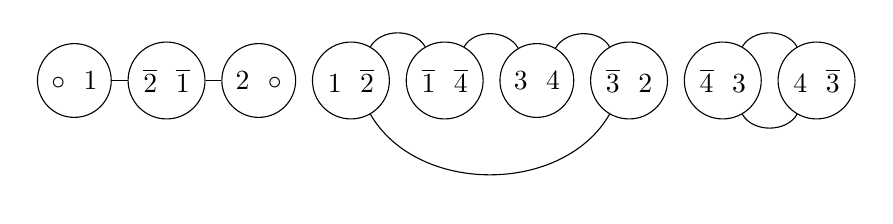
\begin{tikzpicture}
    \matrix[row sep=1mm,column sep=2mm,ampersand replacement=\&] {
      \node[draw,circle] (LA1)  {\paff{\circ}{1}}; \&
      \node[draw,circle] (B2A2) {\pass{2}{1}}; \&
      \node[draw,circle] (B1R)  {\paff{2}{\circ}}; \&
      \node[draw,circle] (A1B2) {\pafs{1}{2}}; \&
      \node[draw,circle] (A2D2) {\pass{1}{4}}; \&
      \node[draw,circle] (C1D1) {\paff{3}{4}}; \&
      \node[draw,circle] (C2B1) {\pasf{3}{2}}; \&
      \node[draw,circle] (D2C1) {\pasf{4}{3}}; \&
      \node[draw,circle] (D1C2) {\pafs{4}{3}}; \\
    };

    \draw (A1B2) to [out=60,in=120] (A2D2);
    \draw (A1B2) to [out=-60,in=-120] (C2B1);

    \draw (B2A2) to [out=0,in=180] (B1R);
    \draw (B2A2) to [out=180,in=0] (LA1);

    \draw (A2D2) to [out=60,in=120] (C1D1);

    \draw (D2C1) to [out=60,in=120] (D1C2);
    \draw (D2C1) to [out=-60,in=-120] (D1C2);

    \draw (C1D1) to [out=60,in=120] (C2B1);

\end{tikzpicture}

\caption{The natural graph of genome  ; it is composed of one path and two cycles.}
\label{fig:NGdef}
\end{figure}



\begin{definition}
    Given an integer , a \emph{cycle} (resp. \emph{path}) in the 
    natural graph of a rearranged duplicated genome is a cycle (resp. path) 
    that contains  edges. If  is even, the cycle (resp. path) is called 
   \emph{even}, and \emph{odd} otherwise.
\end{definition}

\def\EC{\ensuremath{\mbox{EC}}}
\def\OP{\ensuremath{\mbox{OP}}}

Based on the natural graph, a formula for the DCJ halving distance was given in \cite{Mixtacki08}. Given a rearranged duplicated genome  such that the number of even cycles and the number of odd paths in 
are respectively denoted by   and , the  DCJ halving distance of  is:
    

In the case of the BI halving distance, some peculiar properties of the natural graph need to be stated, allowing to simplify the formula of the DCJ halving distance, and leading to a lowerbound on the BI halving distance.


In the following properties, we assume that  is a genome composed of a 
single linear chromosome containing  distinct markers, each one present 
in two copies in . 


\begin{property}
The natural graph  contains only even cycles and paths: 
\label{prop:EC}
\label{prop:1EP}
\begin{enumerate}
\item All cycles in the natural graph  are even.
\item The natural graph  contains only one path, and this path is even.
\end{enumerate}
\end{property}

\begin{proof}
    First, if \aff{a}{x} is a vertex of the
    graph that belongs to a cycle , then there exists an edge between
    \aff{a}{x} and a vertex \asf{a}{y}. These two
    adjacencies are the only two containing a copy of the marker  at the
    first position. So, if we consider the set of all the first markers in
    all adjacencies contained in the cycle , then each marker in this set is
    present exactly twice. Therefore, the cycle  is an even cycle.
  
    Secondly, the graph contains exactly two vertices (adjacencies) containing the
    marker  which are both necessarily ends of a path in . Thus
   there can be only one path in the graph. Since the number of edges in the 
   graph is even and all cycles are even, then the single path is also even. \qed
\end{proof}


We now give a lowerbound on the minimum length of DCJ scenario transforming 
 into a tandem-duplicated genome.

\begin{lemma}
    Let   be the minimum DCJ distance between  and any 
   tandem-duplicated genome. If  contains  cycles then a 
   lowerbound on  is given by:
    
\label{DCJdistLB}
\end{lemma}


\begin{proof}
    First, since all cycles  of  are even and  contains no odd 
    path, 
   then, from the DCJ halving distance formula, the DCJ halving distance of 
      is .

    Now, since any  tandem-duplicated genome can be transformed into 
    a perfectly duplicated genome with one DCJ, then . Therefore, we have .  \qed
\end{proof}

We are now ready to state a lowerbound on the BI halving distance of a rearranged duplicated genome .

\begin{theorem}
    If  contains  cycles, then a lowerbound on the BI halving distance
    is given by: 

\end{theorem}

\begin{proof}

We denote by  the length of a rearrangement scenario .
   Let  be a BI scenario transforming  into a
   tandem-duplicated genome.
    From property \ref{1BIto2DCJ}, we have that  is equivalent to
    a DCJ scenario  such that  . 
    Now, suppose that , then .
    
    This implies . Thus, from Lemma 
   \ref{DCJdistLB} we have  
    which contradicts the fact that  is the minimal number
    of DCJ
    operations required to transform  into a tandem-duplicated genome.

    In conclusion, we always have .  \qed
\end{proof}



\section{Formula for the BI halving distance}
\label{sec:dist}

In this section, we show that the BI halving distance of a rearranged duplicated genome  with  distinct markers such that   contains  cycles is exactly:



In other words, we show that enforcing the constraint that 2 consecutive DCJ have to be equivalent to a BI doesn't change the distance (even though it obviously restricts the DCJ that can be performed at each step of the scenario). 







In
the following,  denotes a rearranged duplicated genome 
constisting in a single linear chromosome with  distinct markers
after the reduction process, and such that  contains  cycles.
We begin by recalling some useful definitions and properties of the DCJ
operations that allow to decrease the DCJ halving distance by  in the resulting genome. 

\begin{definition}
A DCJ operation on  producing genome  is \emph{sorting} if it decreases the DCJ halving distance by : .
\end{definition}

Since the number of distinct markers  is  and , then  contains  cycles. In other words, a DCJ operation is sorting if it increases the number of cycles in   by .

Given  an adjacency of  that is not a double-adjacency,
we denote by  the DCJ operation that cuts adjacencies  and   to form adjacencies  and  , making  a double-adjacency. 

\begin{property}
Let   be an adjacency of  that is not a double-adjacency,
  is a sorting DCJ operation.
\end{property}
\begin{proof}
 increases the number of cycles in   by , by creating a new cycle composed of adjacencies   and  . \qed
\end{proof}

 

















\begin{figure}[!h]
\centering
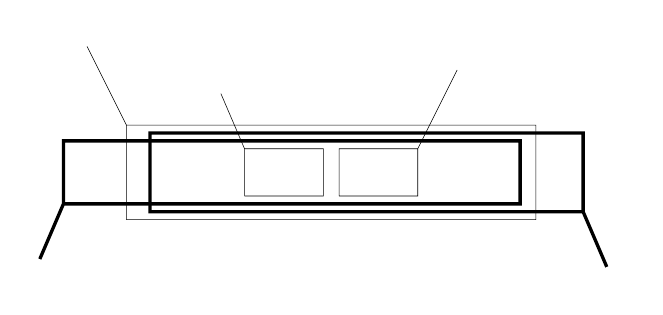
\begin{tikzpicture}
    \matrix[row sep=1mm,column sep=8mm,ampersand replacement=\&] {

\node (L) {}; \&
\node (f2) {}; \&
\node (f1) {}; \&
\node (s2) {}; \&
\node (f3) {}; \&
\node (s1) {}; \&
\node (s3) {}; \&
\node (R) {}; \\
};
\draw[very thin] (0.1,-0.3) -- ++(1,0) -- ++(0,0.6) -- ++(-1,0) --
++(0,-0.6) -- ++(0,0.6) -- ++(1,0) -- ++(0.5,1) node[above]
{};
\draw[very thick] (-3.4,-0.4) -- ++(5.8,0) -- ++(0,0.8) -- ++(-5.8,0)
-- ++(0,-0.8) -- ++(-0.3,-0.7) node[below] {};
\draw[very thin] (-2.6,-0.6) -- ++(5.2,0) -- ++(0,1.2) -- ++(-5.2,0) --
++(0,-1.2) -- ++(0,1.2) -- ++(-0.5,1) node[above] {};
\draw[very thick] (-2.3,-0.5) -- ++(5.5,0) -- ++(0,1) -- ++(-5.5,0) --
++(0,-1) -- ++(5.5,0) -- ++(0.3,-0.7) node[below] {};
\draw[very thin] (-1.1,-0.3) -- ++(1,0) -- ++(0,0.6) -- ++(-1,0) --
++(0,-0.6) -- ++(0,0.6) -- ++(-0.3,0.7) node[above] {};

\end{tikzpicture}
\\

\caption{ , the set of intervals of  depicted as boxes. The two boxes with thick lines represent two 
  overlapping intervals of  inducing a \BI\xspace which 
  exchanges  and .}
    \label{fig:intervaldef}
\end{figure}

\begin{definition}
Let ,  , and   be adjacencies of . The \emph{interval} of the adjacency  , denoted by  is either:
\begin{itemize}
\item the interval  if .  In this case, we denote it by , or
\item the interval  if .
\end{itemize}
\end{definition}

For example, the intervals of the adjacencies in genome  are depicted in Fig \ref{fig:intervaldef}.
Note that, given an adjacency   of ,  if   is a double-adjacency then the interval  is empty, otherwise   is the excision operation that extracts the interval  to make it circular, thus producing the adjacency .



Two intervals   and  are said \emph{overlapping} if
their intersection is non-empty, and none of the intervals is included in the 
other.
It is easy to see, following Property \ref{1BIto2DCJ}, that given two
adjacencies  and  of  such that
 and  are non-empty intervals, the
successive application of  and  is
equivalent  to a BI operation if and only if  and
 are overlapping. Note that in this case neither
, nor   can be double-adjacencies in  since
their  intervals are non-empty. Figure \ref{fig:intervaldef} shows an
example of two overlapping intervals. 


The following property states precisely in which case the successive application of  and  decreases the DCJ halving distance by , meaning that both DCJ operations are sorting.

\begin{property}
Given two adjacencies  and  of , such that 
 and  are overlapping, the successive application of  and  decreases the DCJ halving distance by  if and only if   and .
\end{property}
\begin{proof}
If  and , then the successive application of  and  increases the number of cycles in  by , by creating two new 2-cycles. Otherwise,  first creates a new cycle that is then destroyed by  .
\qed
\end{proof}

We denote by , the set of intervals of all the adjacencies of  that do not contain marker .

\begin{remark}
Note that, if  contains  distinct markers, then there are  adjacencies in  that do not contain marker ,  defining  intervals in  .
\label{maxEdges}
\end{remark}

\begin{definition}
Two  intervals  and  of  are said \emph{compatible} if they are overlapping and   and .
\end{definition}



In the following, we prove the BI halving distance formula by showing that if genome  contains more than three distinct markers, ,  then there exist two compatible intervals in , and if  or  then  and .
This means that there exists a \BI ~halving scenario  such that all \BI ~operations in , possibly excluding the last one, are equivalent to two successive sorting DCJ operations.






From now on, until the end of the section,
 is an adjacency of  that is not a double-adjacency,  is a genome consisting in a linear chromosome  and a circular chromosome , obtained by applying the \emph{sorting DCJ}, , on .

If there exists an interval  in  compatible with  , then applying  on  consists in the integration of the circular chromosome  into the linear chromosome  such that the adjacency  is formed.
Such an \emph{integration} can only be performed by cutting an adjacency  in  and an adjacency  in  (or inversely) to produce adjacencies  and .  This means that there must be an adjacency \aff{x}{y} in either  or  such that  is in  and  in  or inversely.
Hence, we have the following property :



\begin{property}
 \emph{cannot} be reintegrated into  by
applying a sorting DCJ,  , on  if and only if either:

\begin{itemize} 
\item[(1)] for any adjacency  in 
  (resp. ), markers  and  are in
   (resp. ), or

\item[(2)] for any adjacency  in  (resp. ), markers  and  are also in  (resp. ). \end{itemize}

\label{formuleENR}
\end{property}
\begin{proof}
If there exists no  adjacency  in  such that  is in  and  in  or inversely, then  necessarily satisfies either , or . \qed
\end{proof}






\begin{definition}
An interval  in   is called
\emph{interval of type 1} (resp. \emph{interval of type 2}) if  produces a genome  satisfying configuration   (resp.  configuration ) described in Property \ref{formuleENR}.
\end{definition}


For example, in genome  ,   is of type 1 as   produces genome 
 ;   is of type 2 as   produces genome  .

Now we give the maximum numbers of intervals of type 1 and type 2 that can be contained in genome .

\begin{lemma}
The maximum number of intervals of type 1 in  is 2.
\label{maxType1}
\end{lemma}

\begin{proof}
First, note that there cannot be two intervals  and  of  
such that , and both   and  are of type 1.
Now, if  is an interval of type 1, there can be at most two different 
adjacencies  and  such that 
. In this case  necessarily has a chromosome of the form  or .
Therefore, there are at most two intervals of type 1 in .   \qed




\end{proof}

\begin{lemma}
The maximum number of intervals of type 2 in   is .
\label{maxType2}
\end{lemma}

\begin{proof}
First, note that for two adjacencies  and  in  that 
do not contain marker , if  is of type 2 then  
cannot be of type 2.
Now, there is only one marker  such that   is an adjacency 
of . Let  be the adjacency of  having  as first marker, 
then at most half of the intervals in  can 
be of type 2.
Therefore, there are at most  intervals of type 2 in .   \qed








\end{proof}


\begin{theorem}
If  contains  cycles, then the BI halving distance of 
    is given by: 

\label{th:distance}
\end{theorem}

\begin{proof}




    Since there are  intervals in , and at
    most  are of type  or , then if  is a genome
    containing more than three distinct markers , then
     and there exist two compatible intervals in
     inducing a BI operation that decreases the DCJ
    distance by .







Next, we show that if  or , then  and .
 
If , then the genome can be written, either as
, in which case a BI
can swap  and  to produce a tandem-duplicated
genome, or as , in
which case a BI can swap  and  to produce a
tandem-duplicated genome.

If , then the genome has two double-adjacencies to be
constructed, of the form , , with 
and  being two adjacencies already present in the genome
such that  or  and  and 
are distinct markers. One can rewrite  and  as
single markers since they will not be splitted, which makes a genome
with 4 markers such that at most 2 are misplaced. Then, a single BI
can produce a tandem-duplicated genome.

Now, it is easy to see to see that if   or , then . Finally, if   or , then , otherwise we would have   which would imply, as  consists in a single linear chromosome, .
In conclusion, if  then there exist two compatible intervals in  , otherwise if   or , then  and  . Therefore . \qed


\end{proof}





\section{Sorting algorithm}
\label{sec:scenario}



In Section \ref{sec:dist}, we showed that if a genome  contains more than 
three distinct markers after reduction then there exist two compatible 
intervals in  inducing a BI to perform.
If  contains two or three distinct markers then the BI to perform can be 
trivially computed.
Thus the main concern of this section is to describe an efficient algorithm 
for finding compatible intervals when .


As in Section \ref{sec:dist}, in the following,  denotes a genome consisting 
of  distinct markers after reduction. 
It is easy to show that the set of intervals 
 can be built in  time and space complexity.




We now show that finding 2 compatible intervals in   can be done in  time and space complexity.


\begin{property}
If  , then all the smallest intervals in  that are not of type 2 admit compatible intervals.
\label{smallestOK}
\end{property}

\begin{proof}











    Let  be a smallest interval that is not of type 2 in
    . As  is not of type 2, then  has compatible
    intervals if  is not of type 1.

Let us suppose that  is of type 1, then for any adjacency  such 
that markers  and  are not in ,   and  are in , 
and then  is strictly included in  and  can't be of 
type 2. Such adjacency does exist as there are  markers not included in .
Therefore  cannot be a smallest interval that is not of type 2.
\qed
\end{proof}











We are now ready to give the algorithm for sorting a duplicated genome  into a tandem-duplicated genome with  BI operations.



\begin{algorithm}                      \caption{Reconstruction of a tandem-duplicated genome}          \label{alg1}                           \begin{algorithmic}[1]                    
\WHILE{ contains more than  markers}
\STATE Construct 
\STATE Pick a smallest interval  that is not of type 2 in 
\STATE Find an interval  in  compatible with 
\STATE Perform the \BI ~ equivalent to  followed by 
\STATE Reduce 
\ENDWHILE
\IF{ contains  or  markers}
\STATE Find the last BI operation and perform it
\ENDIF
\end{algorithmic}
\end{algorithm}



\begin{theorem}

Algorithm \ref{alg1} reconstruct a tandem-duplicated genome with a BI scenario of length  in  time and space complexity.
\end{theorem}

\begin{proof}
Building  and finding two compatible intervals can be done in  time and space complexity. It follows that the while loop in the algorithm can be computed in  time and space complexity.



Finding and performing the last \BI~operation when   can be done in constant time and space complexity.

Moreover, all \BI~ operations, possibly excluding the last one, are computed as 
pairs of sorting DCJ operations, which ensures that the length of the scenario 
is . \qed
\end{proof}


\section{Conclusion}

In this paper, we introduced the BI halving problem. We use the DCJ model
to simulate BI operations and we showed that it is always possible to choose two consecutive 
sorting DCJ operations such that they are equivalent to a BI operation.
We thus provide a quadratic time and space algorithm to obtain a
most parsimonious scenario as any computed BI scenario is in fact an optimal DCJ scenario.
Finally, one direction for further studies of variants of the BI halving problem is to consider multichromosomal
genomes and BI operations acting on more than one chromosome.
\bibliographystyle{plain} 
\bibliography{article1}

\end{document}
